\documentclass{article} % For LaTeX2e
\usepackage{iclr2018_conference,times}
\usepackage{hyperref}
\usepackage{url}
\usepackage{graphicx}
\usepackage{natbib}


\title{(tentative) Learning Neural Markers of Schizophrenia Disorder Using Recurrent Neural Networks}

% Authors must not appear in the submitted version. They should be hidden
% as long as the \iclrfinalcopy macro remains commented out below.
% Non-anonymous submissions will be rejected without review.

\author{Antiquus S.~Hippocampus, Natalia Cerebro \& Amelie P. Amygdale \thanks{ Use footnote for providing further information
about author (webpage, alternative address)---\emph{not} for acknowledging
funding agencies.  Funding acknowledgements go at the end of the paper.} \\
Department of Computer Science\\
Cranberry-Lemon University\\
Pittsburgh, PA 15213, USA \\
\texttt{\{hippo,brain,jen\}@cs.cranberry-lemon.edu} \\
\And
Ji Q. Ren \& Yevgeny LeNet \\
Department of Computational Neuroscience \\
University of the Witwatersrand \\
Joburg, South Africa \\
\texttt{\{robot,net\}@wits.ac.za} \\
\AND
Coauthor \\
Affiliation \\
Address \\
\texttt{email}
}

% The \author macro works with any number of authors. There are two commands
% used to separate the names and addresses of multiple authors: \And and \AND.
%
% Using \And between authors leaves it to \LaTeX{} to determine where to break
% the lines. Using \AND forces a linebreak at that point. So, if \LaTeX{}
% puts 3 of 4 authors names on the first line, and the last on the second
% line, try using \AND instead of \And before the third author name.

\newcommand{\fix}{\marginpar{FIX}}
\newcommand{\new}{\marginpar{NEW}}

%\iclrfinalcopy % Uncomment for camera-ready version, but NOT for submission.

\begin{document}


\maketitle

% Outline: 
% 1. Introduction: RNNs and CNNs being used for variety of recognition and diagnosis tasks. Problem with previous attempts
% to learn features from brain imaging data (fmri). High variability in brain responses across individuals.
% 2. Related Work: previous work on frmi, previous work to learn from videos, previous work to diagnose schizophrenia 
% 4. Methods
%   4.1 dataset
%   4.2 recurrent-convolutional neural nets for feature learning from fmri segments
% 5. Experiments: 
%   5.1 effectiveness of RNNs and R-CNNs to learn discriminative features from fmri
%	  5.2 generalizability of learned features across datasets
% 6. Discussion
% 7. Conclusion

\begin{abstract}
... Here we propose a new method based on recurrent-convolutional neural networks to automatically learn useful representations from short segments of fMRI recordings...
\end{abstract}

\section{Introduction}
A key challenge in dealing with neuroimaging data comes from the inter- and intra-subject variability that any robust diagnosis system should be robust to. A prominent cause of these variabilities are due to small differences in the functional cortical mapping between individuals which calls for neural markers that are position and scale invariant.

\section{Related Work}



\section{Methods}

\subsection{Dataset}
One scan was captured every 2 seconds. Each session (??) consists of a single fMRI scanning session which lasted for almost 5 minutes (??). Data from each session was split to windows of 32 or 128 seconds which formed the samples used for training, evaluation, and test.  

\subsection{Recurrent-Convolutional Neural Networks}
We compared accuracy of recurrent neural networks (LSTM model) and recurrent-convolutional nerual networks (R-CNN) with baseline classifiers to learn discriminative features for the problem of distinguishing normal and schizophrenic individuals. We tried several different architectures consisting of LSTMs as well as R-CNNs. The input data was structured as a 3-dimensional tensor (3D brain scans). 

\textbf{Baseline Classifier}: We used a $L_1$-regularized logistic regression model and Support Vector Classifier (SVC) applied on voxel activations as the baseline models to compare against. Both of these models were trained on voxel values on all time-frames (did we do this??). 

\textbf{LSTM model}: All voxel values are reshaped into a vector and fed directly into a two-layer forward LSTM model. LSTMs are known for their ability in learning long-term dependencies between inputs. In this model the spatial relationship between voxels are ignored and LSTM learns the temporal relationship between activations in different voxels. 

\textbf{Conv-LSTM model}: 3-D activations for each time frame were fed into a 3D CNN. We used 3-dimensional convolutions followed by max-pooling to extract position and scale independent features that would generalize across individuals. Identical networks were used to process each time-frame with shared weights between them. Outputs of each CNN were then reshaped into a vector that was fed as input to the LSTM network at each time step. Figure-\ref{fig1} shows an overview of the recurrent-convolutional network used here. CNN part learns 3-D features that are invariant to translation and scaling and reduces the dimension of the input space before feeding it into LSTM. 

A batch size of 64 was used for all models. Larger convolutional models were trained synchronously on 16 GPUs. In both cases we experimented with varying number of time-frames included in each sample (i.e. 16 and 64).

\subsection{Training Details}
\label{training_details}
We used Adam optimizer with default parameter settings ($\beta_1=0.9, \beta_2=0.999, \epsilon=10^{-8}$). We included dropout in the input and outputs of the LSTM cells \citep{Zaremba2014} which contained most of the tunable parameters in our models. 

10-fold cross-validation was used to evaluate the performance for each proposed model. $l_2$ regularizer was used on all convolutional and fully connected weights. 
3D-convolutions of size $3\times3\times3$ with stride 1 were used. Each block of convolutions were followed by a maxpool layer of size 2 and stride 2. Feature map size was dividing by 2 after each maxpool layer. Size of the input to the network was $(53\times64\times37)$.

A different subset of subjects were assigned to the test set for each fold and data from the rest of the subjects were used for training and validation (without overlap between train and validation sets). For training, samples within each batch were generated by randomly selecting time windows from different subjects. All possible time windows of size $T$ from all subjects were used for training, validation and test. For each fold training was done for 10 folds. We used the validation set to for early stopping of training. After each training epoch, performance on the validation set was computed. Training was performed for 10 epochs and test performance was computed for the network state with highest validation score. 



\begin{figure}[t]
\begin{center}
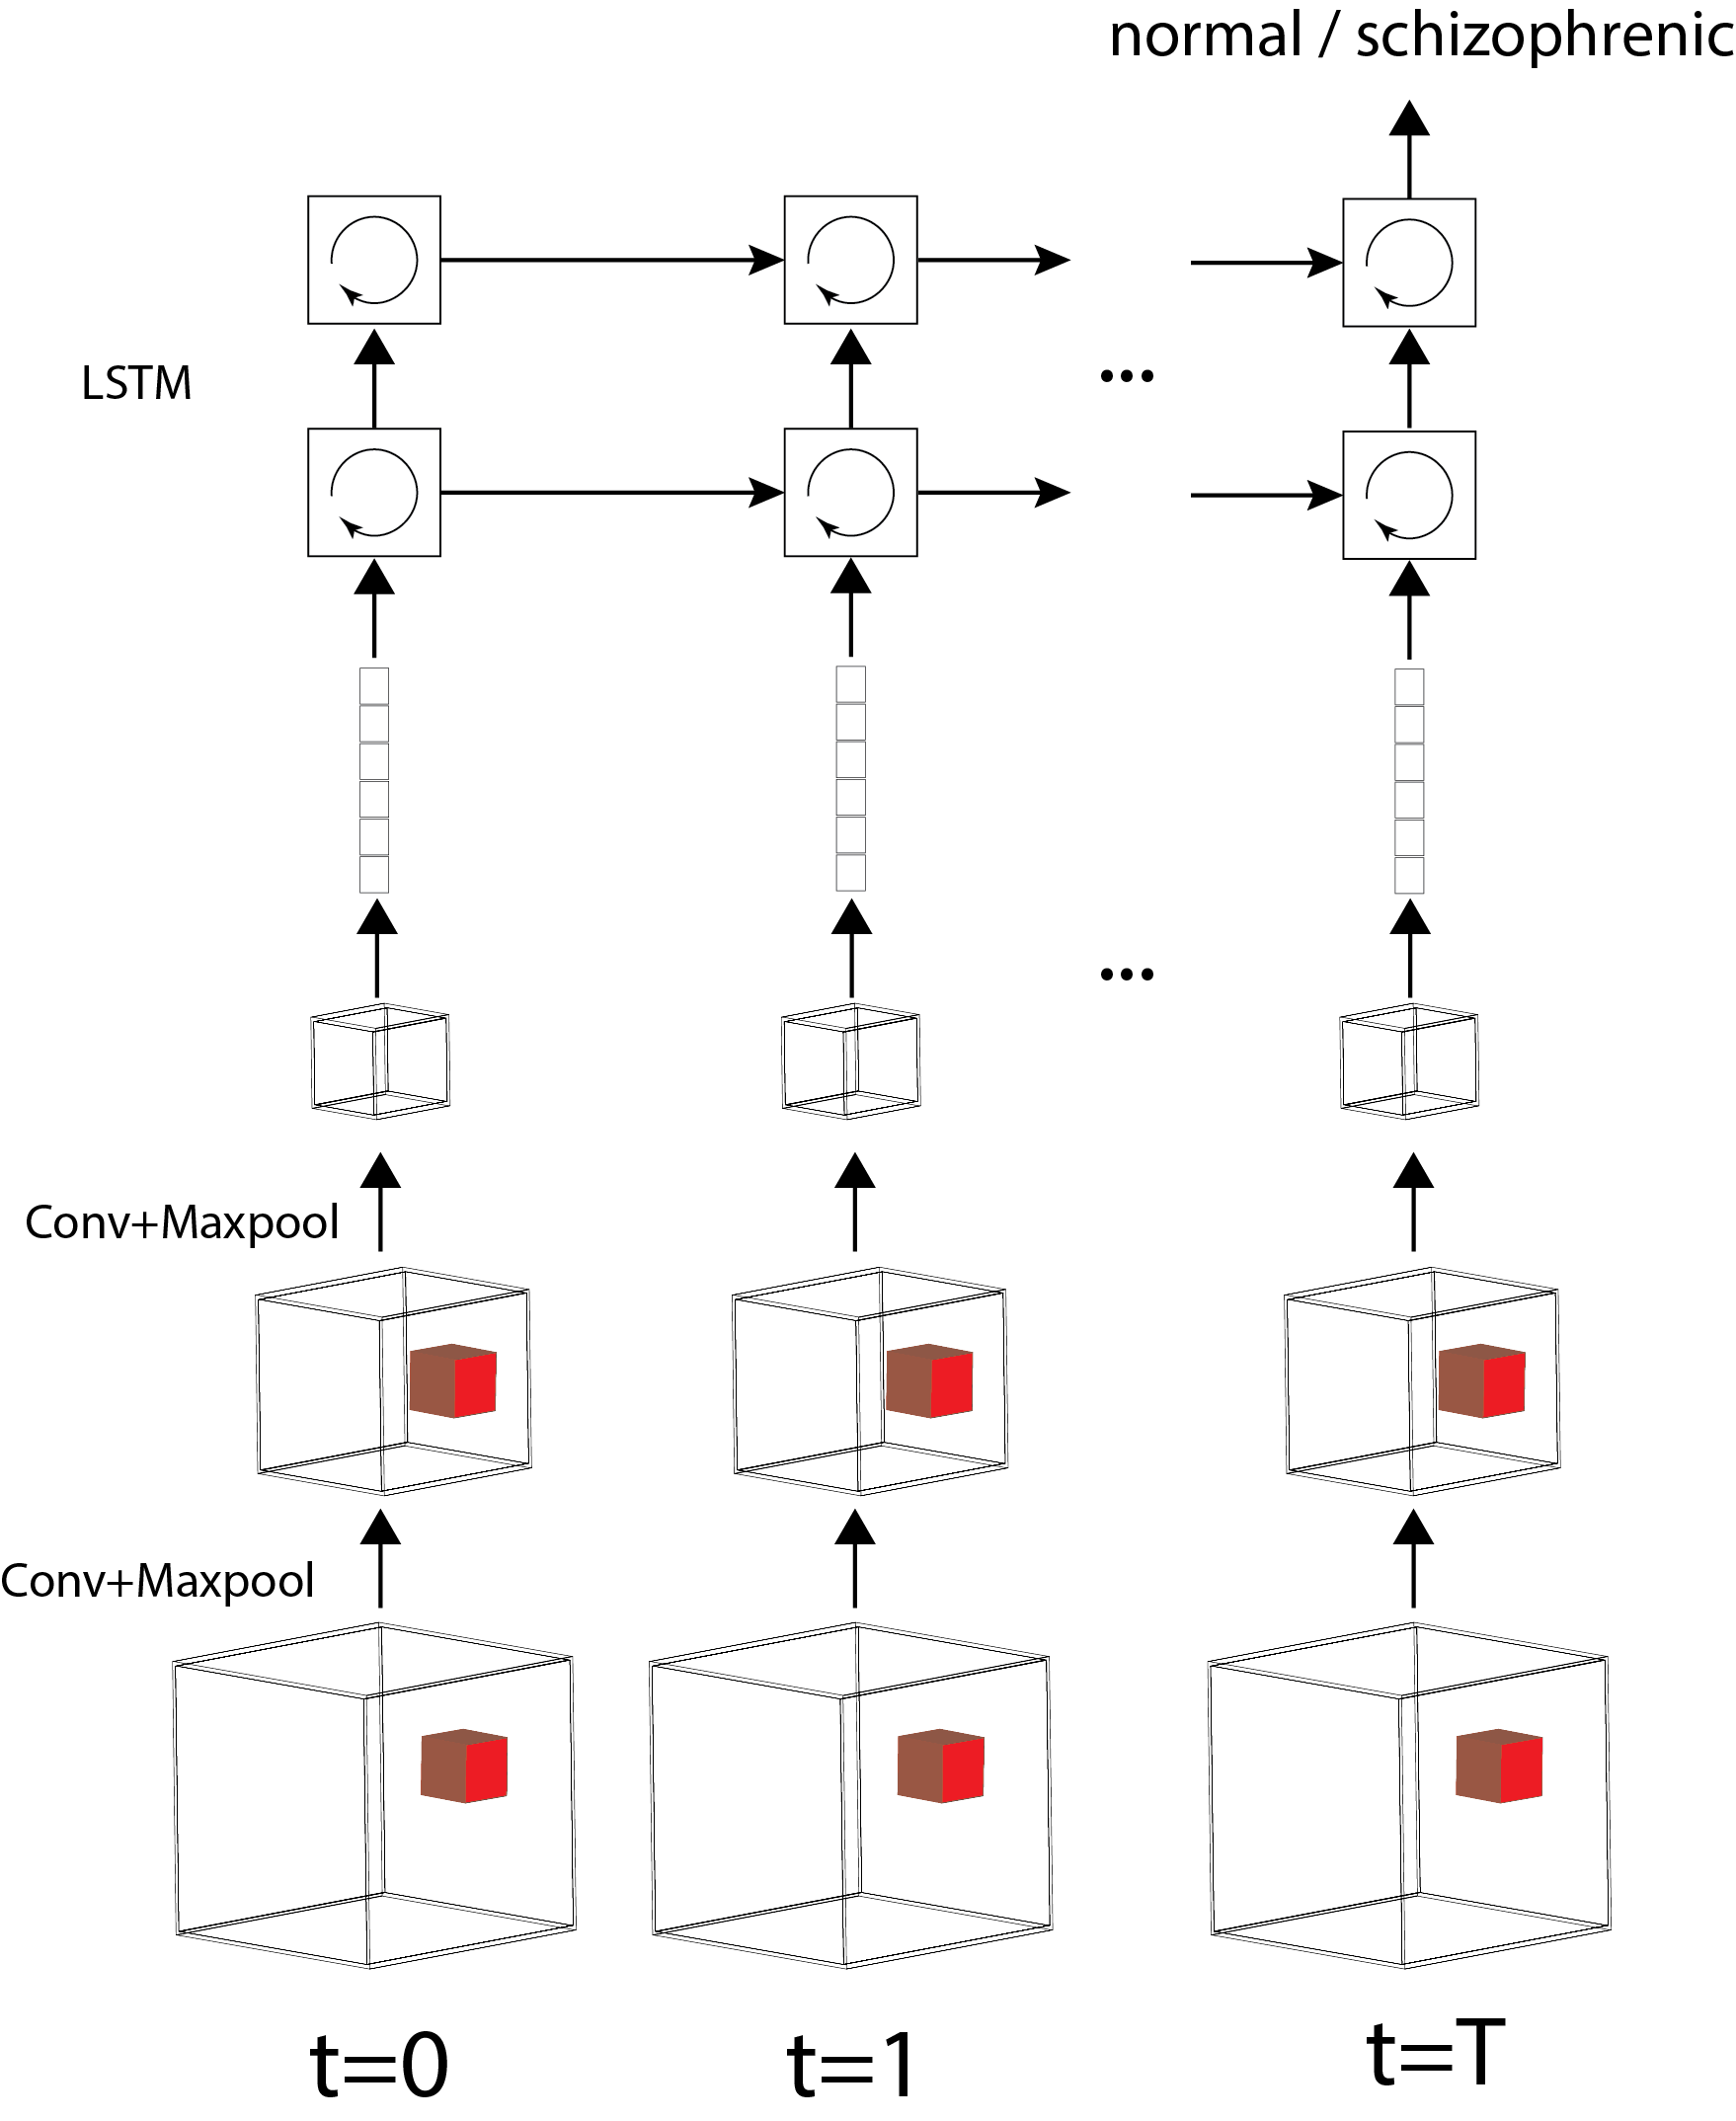
\includegraphics[width=3in]{figures/overview.png}
\end{center}
\caption{Overview of the method used.}
\label{fig1}
\end{figure}

\subsection{Data Preprocessing}
Data preprocessing was done in three steps. (i) For each subject-run the average voxel activation was subtracted; (ii) each subject-run was 

\subsubsection*{Acknowledgments}

Use unnumbered third level headings for the acknowledgments. All
acknowledgments, including those to funding agencies, go at the end of the paper.

\bibliography{iclr2018_conference}
\bibliographystyle{iclr2018_conference}

\end{document}
